\documentclass[11pt]{article}
\usepackage[margin=0.9in]{geometry}
\usepackage{amsmath,amssymb}
\usepackage{booktabs}
\usepackage{enumitem}
\usepackage{tikz}
\usetikzlibrary{positioning}
\usepackage[hidelinks]{hyperref}
\setlist{nosep,leftmargin=1.4em}
\setlength{\parskip}{3pt}
\setlength{\parindent}{0pt}

\title{\vspace{-1.5em}Certified Conditional Cooperation Between Programs:\\ What We Tried, What We Learned, and When to Return}
\author{Findings memo for Cam and collaborators \quad (\texttt{\~{}/dev/diag}, November 2026)}
\date{\vspace{-2.5em}}

\begin{document}
\maketitle

\begin{center}
\fbox{\parbox{0.94\linewidth}{\small
\textbf{Status: parked.} We built a machine-checked scheme in which programs cooperate in the Prisoner's Dilemma by exchanging proof certificates, and it works. Its guarantees, however, rest on an assumption that program-equilibrium results generally leave implicit: a \emph{binding executor} that runs the code each player shows and delivers both moves. With such an executor, a plain escrow contract already provides the same guarantees. Without one, no scheme provides them exactly, and the best available is an $\varepsilon$ of exploitability. Our approach would therefore matter only where execution is binding but there is no shared contract, and each agent keeps its own code. We could not name such a setting. \emph{Return if someone can} (Section~6).}}
\end{center}

\section*{1\quad The goal}

Open-source game theory studies agents that read each other's source code before acting. In the one-shot Prisoner's Dilemma (payoffs $T > R > P > S$: temptation, reward, punishment, sucker), this allows \emph{conditional} cooperation. The best-known example is FairBot, which cooperates if it can prove that its opponent cooperates with it. By Löb's theorem, two FairBots cooperate even when written differently. But FairBot has to \emph{search} for that proof. Exhaustive search over proofs of length $B$ costs about $|\Sigma|^B$, which is affordable only up to $B \approx 20$--$28$, while Critch's bounded version of the argument needs $B \gtrsim 10^4$.

Our idea was to replace search with checking, as in proof-carrying code. Players agree in advance on a \emph{standard} $K$, and each submits its program with a \emph{certificate}: a proof that the program satisfies $K$. An LLM writes both. At play time each side runs one certificate check and no search.

\section*{2\quad What we built}

The difficulty is self-reference. $K$ must say ``I cooperate with you exactly when your certificate proves that \emph{you} satisfy $K$''. Naive versions either regress (a proof about a proof about\ldots) or fall into the \emph{Löb trap}: if the logic may reason about its own checker, every program becomes a member, DefectBot included. We avoid both by defining $K$ with the diagonal lemma instead of Löb's theorem, and by giving the object logic $S$ no reflection rule about its own checker.

Everything is formalized in Lean~4, with no \texttt{sorry} and only Lean's three standard axioms.\footnote{A small DSL with a fuel-bounded interpreter \texttt{run} (each operation is charged the size of the value it builds, so values stay bounded by fuel: \texttt{eval\_sz\_le}); the logic $S$ with checker \texttt{check} (\texttt{check\_sound}); \texttt{theoremA}, \texttt{theoremB}, \texttt{exclusivity}. CertBot's certification and tournament outcomes are kernel-checked with \texttt{unseal} and \texttt{decide +kernel}, with no \texttt{native\_decide} or \texttt{\#eval}. Details and \texttt{\#print axioms} output are in \texttt{PROGRESS.md}.} The checker is sound. Two certified members cooperate (Theorem~A), and a certified member is never exploited (Theorem~B). A one-way variant $K'$ comes with an exclusivity theorem: no program satisfies both $K$ and $K'$, so a $K$-member and a $K'$-member defect against each other even though both are ``cooperative''. Certificates range from about 1.7k to 50k in size, and a full game takes about 5\,ms. In a pilot, an LLM wrote 8 of 8 certified members (6 on the first attempt), and the checker accepted none of 6 adversarial candidates. The generator was the same model that built the system, so the pilot is not independent evidence.

The construction works. What it lacked was a reason why anyone needs it, and the rest of the project was a search for one.

\section*{3\quad What we found}

\textbf{Necessity does not single out certificates.} We first tried to show that the approach is forced: if P $\neq$ NP, no fast agent is both \emph{fair} (cooperates whenever a short proof of the opponent's cooperation exists) and \emph{unexploitable}. Our Lean version took its two hard steps as hypotheses, and with a fixed fuel cap one of them is false for large inputs. Proving them inside $S$ would have needed induction and many more sessions. That effort turned out to be beside the point: a simple diagonal argument with Contrarian (``play the opposite of what you play against me'') shows unconditionally that no agent whose runs have short proofs is both fair and unexploitable. It is folklore-level (Anderlini 1990; Barasz et al., \S5), and it constrains \emph{every} feasible approach, so it cannot argue for ours.

\textbf{Zero exploitability is not a requirement.} If necessity cannot justify our criteria, they have to justify themselves, and unexploitability does not. Oesterheld's $\varepsilon$-grounded FairBot is already an equilibrium: defecting against it earns about $\varepsilon T + (1-\varepsilon)P < R$ for small $\varepsilon$. What survives is what Theorems A and B say together: a \emph{verifiable conditional commitment}, ``I cooperate if and only if you make the same commitment''.

\textbf{Even that commitment needs an executor.} Theorems A and B, like every program-equilibrium result we know of, assume that the code each player shows is the code that runs and that both moves are delivered. Making the assumption explicit splits the problem (Figure~\ref{fig:executor}). \emph{With} a binding executor, such as a smart contract or a referee, a plain escrow contract (``both commit, then both cooperate'') already gives A and B; this is Monderer and Tennenholtz's mediator. \emph{Without} one, the guarantee fails in a simple way. Certified agent $b$ blocks its own incoming channel. It never receives $a$'s certificate, so it defects, exactly as $K$ prescribes. Meanwhile $a$ receives $b$'s certificate and cooperates, and is exploited. Signed receipts only move the problem one level up. This is the fair-exchange impossibility (Even and Yacobi; Pagnia and Gärtner) in strategic form, and its known escapes, collateral and gradual release, cost an $\varepsilon$ of exploitability: the same price $\varepsilon$-grounding already pays.

\begin{figure}[t]
\centering
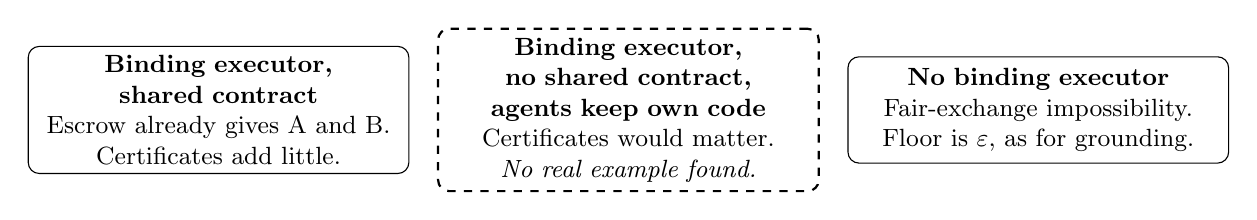
\begin{tikzpicture}[box/.style={draw,rounded corners,align=center,font=\small,text width=4.6cm,minimum height=1.35cm}]
\node[box] (a) {\textbf{Binding executor, shared contract}\\ Escrow already gives A and B.\\ Certificates add little.};
\node[box,right=0.35cm of a,dashed,thick] (b) {\textbf{Binding executor, no shared contract, agents keep own code}\\ Certificates would matter.\\ \emph{No real example found.}};
\node[box,right=0.35cm of b] (c) {\textbf{No binding executor}\\ Fair-exchange impossibility.\\ Floor is $\varepsilon$, as for grounding.};
\end{tikzpicture}
\caption{Where certificate-based cooperation could matter. Only the dashed middle regime distinguishes our approach, and we could not populate it.}
\label{fig:executor}
\end{figure}

\section*{4\quad The open question}

So certificates have no regime of their own unless the middle box of Figure~\ref{fig:executor} is occupied. That box is where our one distinctive feature, \emph{semantic membership}, pays off. Under it, any program \emph{proved} to honor $K$ is a member, rather than one exact program (CliqueBot) or one escrow address. The bare program-equilibrium model sits in the box by definition, but it is a model, not a deployment. The most plausible real candidate is hardware-governance commitments of the flexHEG kind (``if the other party makes the same commitment''), which we have not examined. In hindsight, most of our effort (the necessity theorem, about 135 literature searches) went to questions that do not bear on this one.

\section*{5\quad Paths to a paper}

The answer to that question decides which paper, if any, exists.

\textbf{If the box stays empty: the hidden-assumption note.} The finding of Section~3 is itself the strongest result. Unexploitable conditional cooperation between programs \emph{is} fair exchange: with an executor, escrow suffices; without one, $\varepsilon$ is the floor; Critch, Oesterheld and certificates become points on one map. The cooperative-AI literature lists checkable conditional commitments as open (DiGiovanni, Clifton and Macé 2025, for example, leave template checking to future work), so that audience may not know the reduction. The risk is that cryptographers consider it folklore. Our searches found no written version, but they were snippet-level and confabulated at least one source, so that absence is weak evidence.

\textbf{In either case: a theory note} for open-source game theory. Shipped proofs plus the diagonal lemma give cooperation with no proof search and no Löb, all machine-checked. It is modest, and the artifact exists. The nearest verified work is Duclaux et al.\ 2026 (Lean proofs of pairwise outcomes, found offline by search) and Ondras 2026 (a Lean handshake that relies on a trusted attestation step). Peters and Szentes 2012 have diagonal contracts over program codes, but match codes exactly rather than checking proofs (per our literature synthesis; not re-read).

\textbf{If the box is occupied: a full paper on the construction.} It would also need an LLM run with an independent model and an answer to interoperation between different standards, since $K$- and $K'$-members currently defect against each other.

\section*{6\quad When to pick this up}

\begin{center}
\small
\begin{tabular}{@{}p{0.40\linewidth}p{0.55\linewidth}@{}}
\toprule
\textbf{Resume if\ldots} & \textbf{Cheapest test} \\
\midrule
A real setting has binding execution but no shared contract, and agents keep their own code & Spend 30 minutes trying to name one, starting with flexHEG. Then check whether a single ``CliqueBot-as-escrow'' contract emulates it; if it does, the case fails. \\
Nobody has written ``program equilibrium = fair exchange'' & One hour of searching with opened sources only (Harrenstein 2007; Katz 1991; rational fair exchange), and one email to Oesterheld or DiGiovanni. \\
Someone has a real use for template checking & Ask DiGiovanni, Clifton and Macé what they intended it for. \\
\midrule
\multicolumn{2}{@{}p{0.96\linewidth}@{}}{\textbf{Stop if} the reduction is already known \emph{and} no middle-regime setting turns up. Then archive the Lean repository and post, at most, a short note.}\\
\bottomrule
\end{tabular}
\end{center}

If we return, settle the criteria and whether an executor is assumed \emph{before} proving theorems; we did it the other way round. Treat any literature claim without an opened source as unverified. The Lean development, the literature corpus (about 110 reports, in \texttt{research/related\_work/}) and the record of every hypothesis tried (\texttt{research/OUTLINE\_2026-11-18.md}) are reusable whatever we decide.

\end{document}
